\documentclass[a4paper,oneside,11pt]{book}

% Package dasar
\usepackage[utf8]{inputenc}     % untuk karakter UTF-8
\usepackage[T1]{fontenc}        % encoding font
\usepackage{graphicx}
\usepackage{titling}
\usepackage{titlesec}
\usepackage[backend=biber,style=ieee]{biblatex}
\addbibresource{ref.bib}

% Package tambahan untuk layout dan formatting
\usepackage{geometry}           % untuk margin
\usepackage{setspace}           % untuk spasi baris
\usepackage{fancyhdr}           % untuk header/footer
\usepackage{hyperref}           % untuk link dan bookmark
\usepackage{listings}           % untuk code Python
\usepackage{xcolor}             % untuk warna
\usepackage{float}              % untuk posisi gambar
\usepackage{tocloft}            % Untuk membuat daftar isi menampilkan "Bab 1. Pendahuluan" instead of "1. Pendahuluan",
\usepackage{lipsum}             % untuk lorem ipsum
\usepackage{indentfirst}        % untuk indent paragraf pertama

% Pengaturan layout
\geometry{left=3cm, right=2cm, top=2cm, bottom=2cm}
\onehalfspacing  % spasi 1.5

% Format chapter
\titleformat{\chapter}[hang]
  {\normalfont\huge\bfseries\centering}{\chaptertitlename\ \thechapter.}{1em}{}

% Format code Python
\lstset{
    language=PHP,
    basicstyle=\ttfamily\small,
    keywordstyle=\color{blue}\bfseries,
    commentstyle=\color{gray},
    stringstyle=\color{red},
    numbers=left,
    numberstyle=\tiny,
    frame=single,
    breaklines=true,
    showstringspaces=false,
    xleftmargin=2cm,
    xrightmargin=1cm,
    morekeywords={Route,Controller,Request,Response,Blade,Model,Migration,Artisan,middleware,Auth,extends,section,yield,csrf,foreach,endif}
}

% Pengaturan hyperref
\hypersetup{
    colorlinks=true,
    linkcolor=black,
    filecolor=magenta,
    urlcolor=blue,
    citecolor=red
}

% Info dokumen
\title{Dokumen \\ Proyek Aplikasi Dasar\\
UTS}
\author{Kelompok 21 (SIA WEB)\\
Anggota: \\
1. Nama 1 (123456789)\\
2. Nama 2 (123456789)\\
3. Nama 3 (123456789)\\
4. Nama 4 (123456789)}

\begin{document}

% Title Page
\begin{titlingpage} 
\begin{center}

\vspace{4cm} 
\begin{Large} 
\textbf{\thetitle} \\
\end{Large}
\vspace{2cm}


\includegraphics[height=8cm]{lambang ugm.png}\\ 
\begin{large}
\vspace{2cm} 
\theauthor\\ 
\end{large}

\vspace{2cm}
\begin{Large}
\textbf{Sekolah Vokasi}\\
\textbf{Universitas Gadjah Mada}\\
\textbf{Yogyakarta}\\
\textbf{2025}\\
\end{Large}

\end{center}
\end{titlingpage}

% Header/Footer
\pagestyle{fancy}
\fancyhf{}            % kosongkan header/footer default
\fancyfoot[C]{\thepage} % taruh nomor halaman di footer tengah


% --- Styling Judul Daftar Isi, Gambar, dan Kode ---
\renewcommand{\cfttoctitlefont}{\hfill\normalfont\LARGE\bfseries}
\renewcommand{\cftaftertoctitle}{\hfill}
\renewcommand{\cftbeforetoctitleskip}{1em}
\renewcommand{\cftaftertoctitleskip}{1.5em}

% --- Format Bab di Daftar Isi ---
\renewcommand{\cftchappresnum}{Bab~}
\renewcommand{\cftchapaftersnum}{.}
\renewcommand{\cftchapnumwidth}{3.5em}
\renewcommand{\cftchapfont}{\bfseries}
\renewcommand{\cftchappagefont}{\bfseries}

% --- Spasi dan Estetika ---
\setlength{\cftbeforechapskip}{0.8em} % jarak antar bab
\setlength{\cftbeforesecskip}{0.2em}  % jarak antar subbab
\renewcommand{\cftsecfont}{\normalfont}
\renewcommand{\cftsubsecfont}{\normalfont}

% --- Judul Lokal ---
\renewcommand{\contentsname}{\centering Daftar Isi}
\renewcommand{\listfigurename}{\centering Daftar Gambar}
\renewcommand{\lstlistlistingname}{\centering Daftar Kode}

% --- Gaya Daftar Gambar dan Daftar Kode ---
\renewcommand{\cftloftitlefont}{\hfill\normalfont\LARGE\bfseries}
\renewcommand{\cftafterloftitle}{\hfill}

\tableofcontents

\newpage
% Daftar Gambar
\listoffigures

\newpage


% Contoh gambar
% \begin{figure}[H]
%   \centering
%   \includegraphics[width=0.8\textwidth]{img/HasilTambah.png}
%   \caption{Hasil Tambah Simpanan}
%   \label{fig:hasil_tambah}
% \end{figure}

% Dokumen-Dokumen penting
\chapter{Dokumen}
\section{MVP}
\section{Bisreq}

\newpage
% Use Case
\section{Use Case}

% Subsystem manejer
\subsection{Subsystem: Manajerial}
\begin{figure}[H]
  \centering
  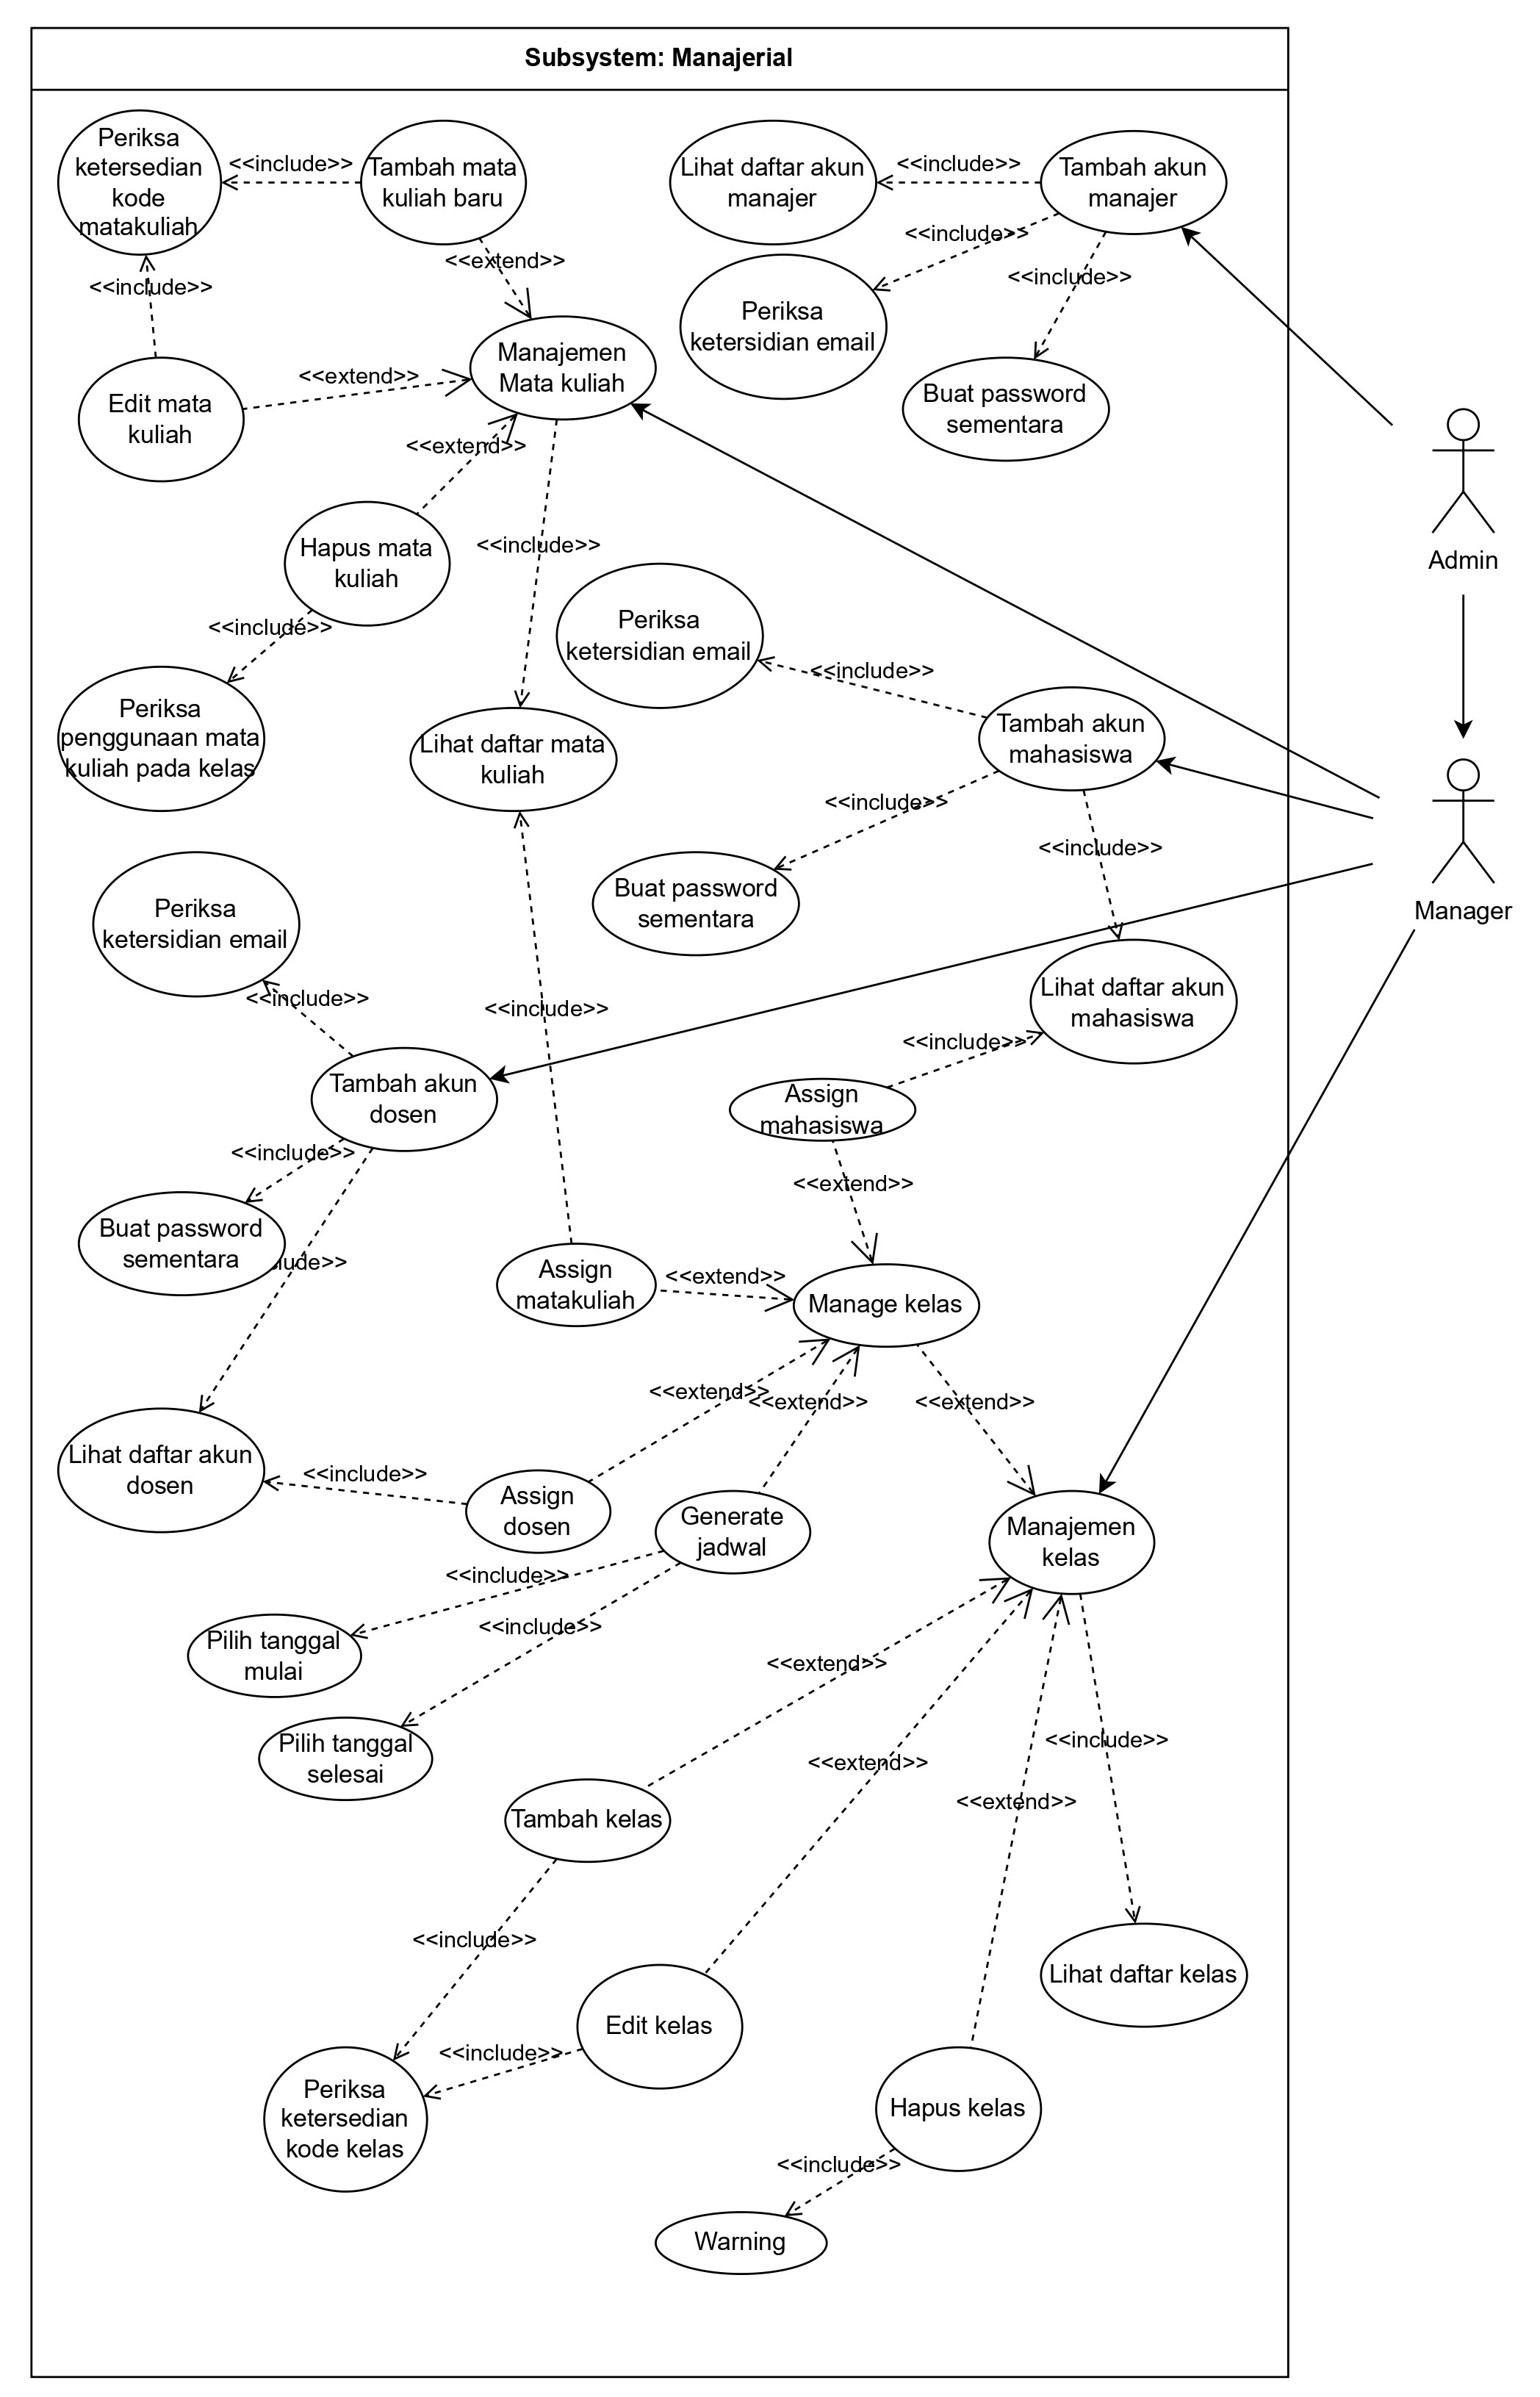
\includegraphics[width=0.8\textwidth]{USECASE/usecasemanajer.jpg}
  \caption{Use Case Manajerial}
  \label{fig:use_case_manajerial}
\end{figure}

\subsubsection{Penjelasan Use Case Manajerial}

Subsystem Manajerial merupakan salah satu bagian inti dalam sistem informasi akademik yang berfungsi untuk mengelola berbagai aspek manajemen perkuliahan, akun pengguna, serta pengaturan kelas dan jadwal. Pada diagram use case \ref{fig:use_case_manajerial} di atas, subsystem ini melibatkan dua aktor utama, yaitu Admin dan Manager, yang memiliki peran berbeda dalam menjalankan fungsionalitas sistem.

\subsubsection{Aktor dan Peran}

\begin{itemize}
  \item \textbf{Admin}: Bertanggung jawab atas pengelolaan akun manajer, dosen, dan mahasiswa, serta memastikan integritas data dan keamanan sistem. Admin dapat menambah akun baru, memeriksa ketersediaan email, dan membuat password sementara untuk pengguna baru.
  \item \textbf{Manager}: Berperan dalam pengelolaan mata kuliah, kelas, dan penjadwalan. Manager dapat menambah, mengedit, dan menghapus mata kuliah serta kelas, mengatur jadwal, dan melakukan assign dosen maupun mahasiswa ke kelas tertentu.
\end{itemize}

\subsubsection{Fitur Utama Subsystem Manajerial}

\begin{enumerate}
  \item \textbf{Manajemen Mata Kuliah:} Fitur ini memungkinkan admin dan manager untuk menambah mata kuliah baru, mengedit, dan menghapus mata kuliah yang sudah ada. Setiap penambahan atau perubahan mata kuliah akan melalui proses validasi, seperti pemeriksaan ketersediaan kode mata kuliah dan penggunaan mata kuliah pada kelas yang sudah berjalan. Hal ini bertujuan untuk menjaga konsistensi data dan mencegah duplikasi atau konflik dalam penjadwalan.
  \item \textbf{Manajemen Akun Pengguna:} Admin dapat menambah akun manajer, dosen, dan mahasiswa. Proses penambahan akun melibatkan pemeriksaan ketersediaan email untuk memastikan tidak ada duplikasi, serta pembuatan password sementara yang dapat diganti oleh pengguna setelah login pertama. Admin juga dapat melihat daftar akun yang sudah terdaftar untuk memudahkan monitoring dan pengelolaan.
  \item \textbf{Manajemen Kelas:} Manager memiliki akses untuk menambah, mengedit, dan menghapus kelas. Setiap kelas yang dibuat harus memiliki kode unik yang diverifikasi oleh sistem. Selain itu, manager dapat melakukan assign dosen dan mahasiswa ke kelas tertentu, serta mengatur jadwal perkuliahan dengan memilih tanggal mulai dan selesai. Fitur generate jadwal membantu manager dalam menyusun jadwal yang optimal dan menghindari bentrok antar kelas.
  \item \textbf{Assign Dosen dan Mahasiswa:} Fitur ini memungkinkan manager untuk mengatur siapa saja dosen dan mahasiswa yang akan mengikuti kelas tertentu. Proses assign dilakukan dengan memperhatikan ketersediaan dosen dan mahasiswa, serta memastikan bahwa tidak ada jadwal yang bertabrakan. Dengan adanya fitur ini, proses pengelolaan kelas menjadi lebih terstruktur dan efisien.
  \item \textbf{Validasi dan Warning:} Setiap proses penambahan atau perubahan data, seperti mata kuliah, kelas, dan akun, akan melalui tahap validasi. Jika ditemukan masalah, seperti kode yang sudah digunakan atau email yang sudah terdaftar, sistem akan memberikan warning kepada pengguna. Hal ini penting untuk menjaga integritas data dan mencegah kesalahan yang dapat berdampak pada proses akademik.
\end{enumerate}


\subsubsection{Alur Interaksi Use Case}

Pada diagram use case \ref{fig:use_case_manajerial} diatas, terlihat adanya relasi <<include>> dan <<extend>> antar fitur. Relasi <<include>> menunjukkan bahwa suatu proses selalu melibatkan proses lain, misalnya setiap penambahan akun pasti melibatkan pemeriksaan ketersediaan email dan pembuatan password sementara. Relasi <<extend>> menunjukkan bahwa suatu proses dapat diperluas dengan fitur tambahan, seperti manajemen kelas yang dapat diperluas dengan fitur generate jadwal atau warning jika terjadi masalah.

\subsubsection{Keamanan dan Efisiensi}

Subsystem Manajerial dirancang dengan memperhatikan aspek keamanan, seperti validasi data dan pembuatan password sementara, serta efisiensi dalam pengelolaan kelas dan jadwal. Dengan adanya fitur-fitur ini, proses administrasi akademik dapat berjalan lebih lancar, terstruktur, dan minim kesalahan.

\subsubsection{Contoh Skenario Penggunaan}

\begin{enumerate}
  \item \textbf{Penambahan Mata Kuliah Baru}: Manager mengakses fitur tambah mata kuliah, memasukkan data mata kuliah, sistem memeriksa ketersediaan kode, jika tersedia maka mata kuliah ditambahkan ke database.
  \item \textbf{Assign Dosen ke Kelas}: Manager memilih kelas yang akan di-assign, memilih dosen yang tersedia, sistem memeriksa jadwal dosen, jika tidak bentrok maka dosen di-assign ke kelas tersebut.
  \item \textbf{Penambahan Akun Mahasiswa}: Admin mengakses fitur tambah akun mahasiswa, memasukkan data mahasiswa, sistem memeriksa email, jika belum terdaftar maka akun dibuat dan password sementara diberikan.
  \item \textbf{Generate Jadwal Kelas}: Manager mengatur jadwal kelas dengan memilih tanggal mulai dan selesai, sistem memeriksa ketersediaan waktu, jika tidak bentrok maka jadwal dibuat dan ditampilkan pada daftar kelas.
\end{enumerate}

\subsubsection{Kesimpulan}

Subsystem Manajerial merupakan komponen penting dalam sistem informasi akademik yang mendukung proses administrasi dan pengelolaan data secara terintegrasi. Dengan fitur-fitur yang lengkap dan terstruktur, subsystem ini membantu admin dan manager dalam menjalankan tugasnya secara efisien, aman, dan akurat. Validasi data, warning, serta relasi antar fitur memastikan bahwa setiap proses berjalan sesuai prosedur dan meminimalisir terjadinya kesalahan. Dengan demikian, subsystem manajerial berperan besar dalam mendukung kelancaran operasional akademik di institusi pendidikan.


% Subsystem login dan usermanajement
\subsection{Subsystem: Login dan User Management}
\begin{figure}[H]
  \centering
  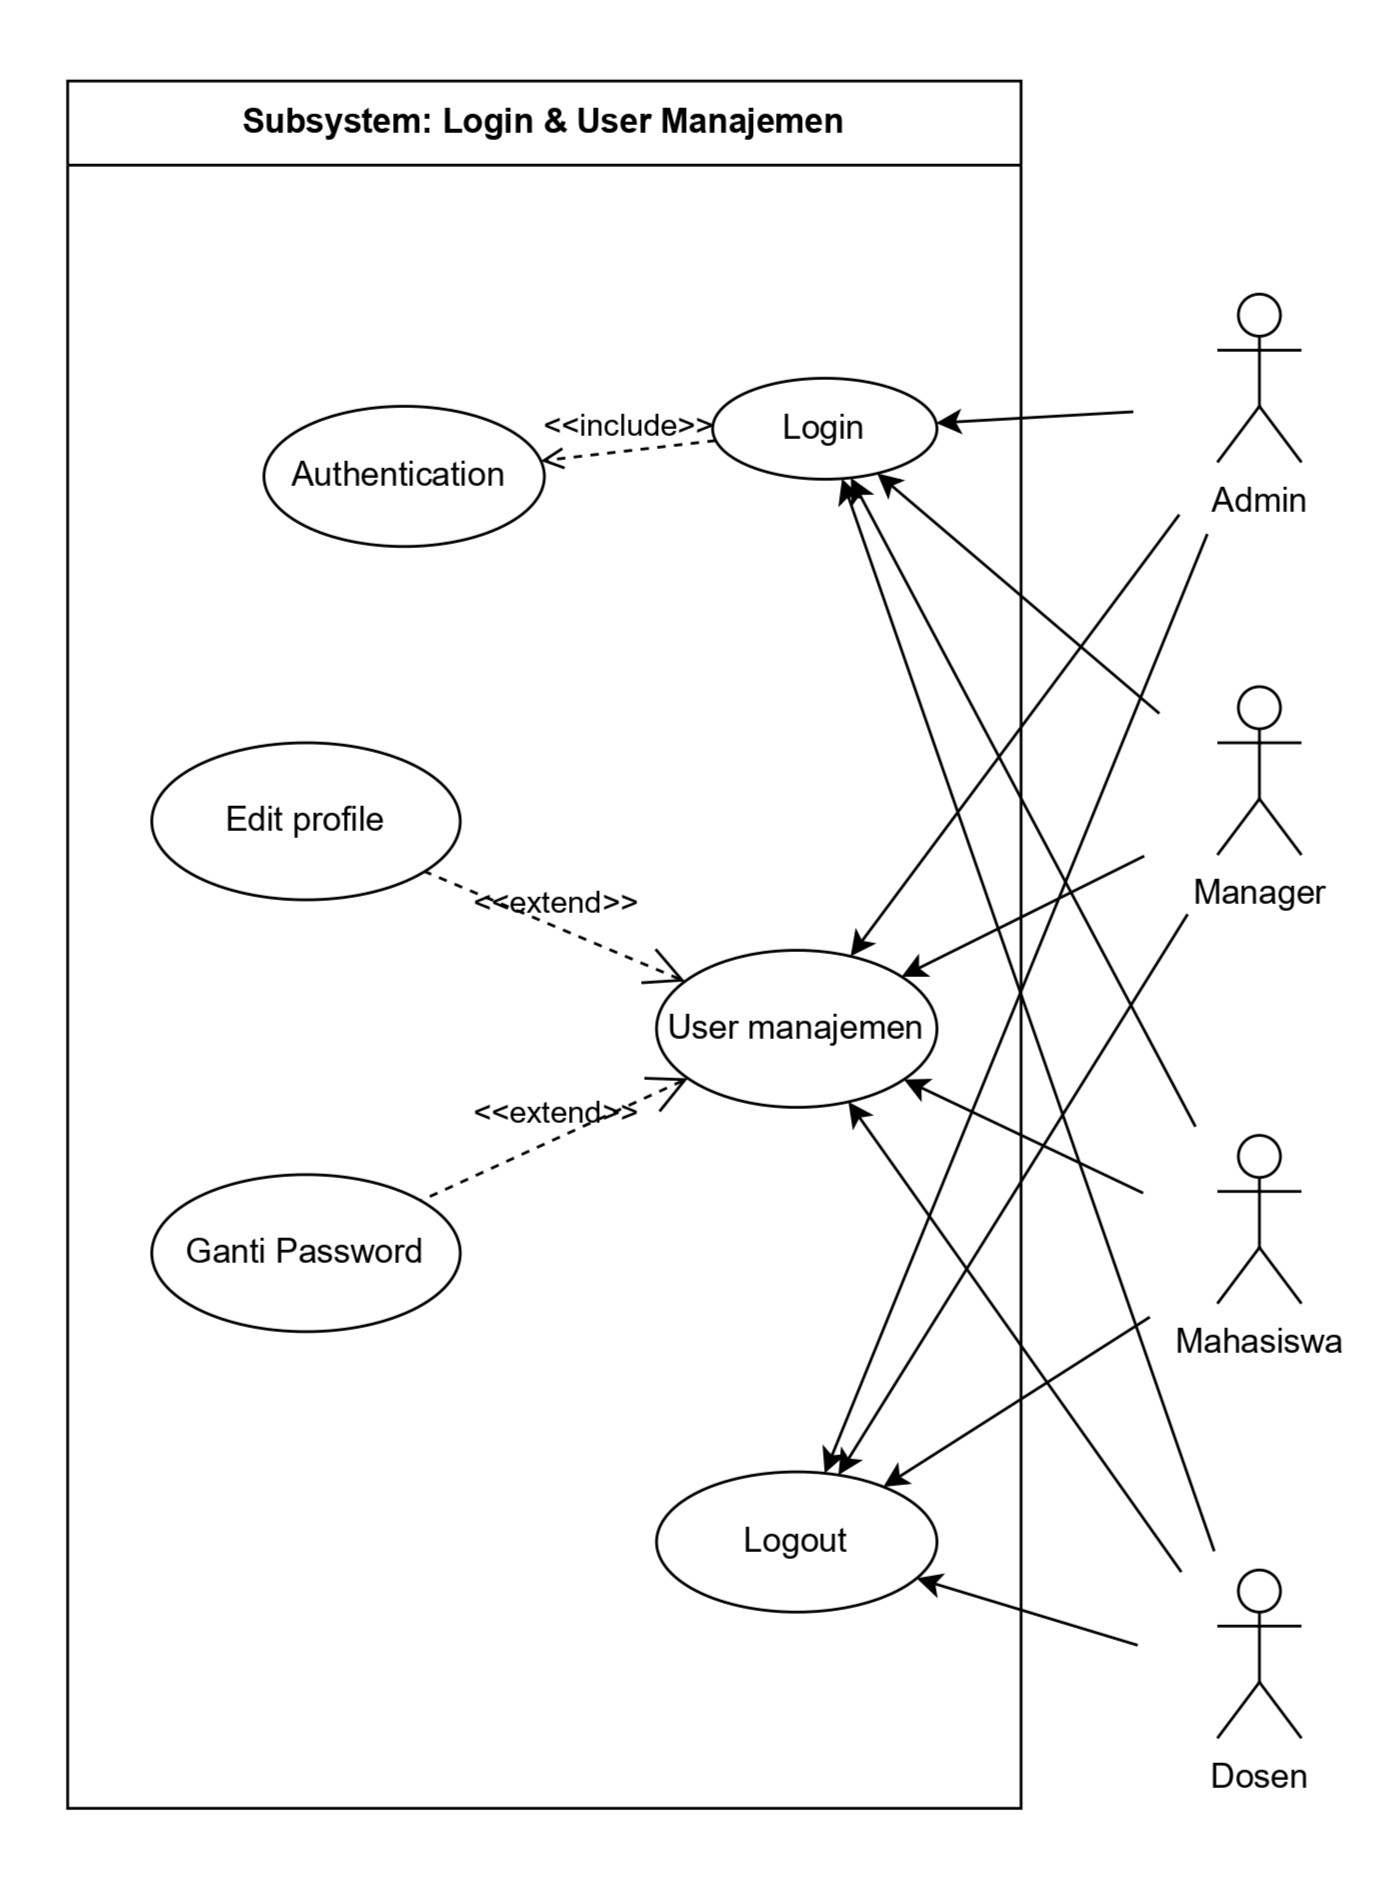
\includegraphics[width=0.8\textwidth]{USECASE/usecaselogin.jpg}
  \caption{Use Case Login dan User Management}
  \label{fig:use_case_login}
\end{figure}

\subsubsection{Penjelasan Use Case Login dan User Management}

Subsystem Login dan User Management merupakan bagian fundamental dari sistem informasi akademik yang bertanggung jawab atas proses autentikasi, pengelolaan identitas pengguna, serta keamanan akses ke seluruh fitur sistem. Pada diagram use case \ref{fig:use_case_login}, subsystem ini melibatkan empat aktor utama, yaitu Admin, Manager, Mahasiswa, dan Dosen, yang semuanya berinteraksi dengan sistem untuk mengakses, mengelola, dan memperbarui data akun mereka.

\subsubsection{Aktor dan Peran}

\begin{itemize}
  \item \textbf{Admin}: Memiliki hak akses penuh untuk mengelola akun seluruh pengguna, melakukan reset password, dan memastikan keamanan sistem.
  \item \textbf{Manager}: Mengelola akun dosen dan mahasiswa, serta dapat memperbarui profil dan password sendiri.
  \item \textbf{Mahasiswa}: Mengakses sistem untuk melihat data akademik, memperbarui profil, dan mengganti password.
  \item \textbf{Dosen}: Mengelola data pribadi, mengakses jadwal, dan melakukan perubahan password sesuai kebutuhan.
\end{itemize}

\subsubsection{Fitur Utama Subsystem Login dan User Management}

\begin{enumerate}
  \item \textbf{Login dan Authentication:} Fitur ini merupakan pintu masuk utama ke sistem. Setiap pengguna harus melakukan login dengan kredensial yang valid. Proses login selalu melibatkan autentikasi, yaitu verifikasi username dan password, serta validasi status akun. Jika autentikasi berhasil, pengguna dapat mengakses fitur sesuai hak aksesnya.
  \item \textbf{User Management:} Setelah login, pengguna dapat mengelola data profil, seperti nama, email, dan informasi kontak. Admin dapat mengelola seluruh akun, termasuk menambah, mengedit, dan menghapus akun pengguna lain. Fitur ini juga mendukung pengelolaan hak akses dan peran pengguna.
  \item \textbf{Edit Profile:} Pengguna dapat memperbarui data pribadi mereka, seperti nama, email, dan foto profil. Fitur ini penting untuk menjaga data tetap akurat dan up-to-date. Proses edit profile dilakukan melalui relasi <<extend>> pada user management.
  \item \textbf{Ganti Password:} Untuk menjaga keamanan, pengguna dapat mengganti password secara mandiri. Proses ini juga dilakukan melalui relasi <<extend>> pada user management. Admin dapat melakukan reset password jika pengguna lupa atau terjadi masalah keamanan.
  \item \textbf{Logout:} Fitur logout memastikan bahwa sesi pengguna berakhir dengan aman, sehingga mencegah akses tidak sah ke data pribadi dan fitur sistem. Semua aktor dapat melakukan logout setelah selesai menggunakan sistem.
\end{enumerate}

\subsubsection{Alur Interaksi Use Case}

Pada diagram use case, terlihat bahwa proses login selalu melibatkan autentikasi (<<include>>), sedangkan user management dapat diperluas dengan fitur edit profile dan ganti password (<<extend>>). Setiap aktor dapat melakukan login, mengelola akun, dan logout sesuai dengan hak akses yang dimiliki. Admin memiliki hak istimewa untuk mengelola seluruh akun dan melakukan reset password, sedangkan pengguna lain hanya dapat mengelola akun mereka sendiri.

\subsubsection{Keamanan dan Efisiensi}

Subsystem ini dirancang dengan fokus pada keamanan data dan efisiensi akses. Proses autentikasi menggunakan enkripsi password dan validasi multi-level untuk mencegah akses tidak sah. Fitur ganti password dan edit profile memberikan fleksibilitas bagi pengguna untuk menjaga keamanan dan akurasi data. Logout yang aman memastikan tidak ada sesi yang terbuka setelah pengguna selesai menggunakan sistem.

\subsubsection{Contoh Skenario Penggunaan}

\begin{enumerate}
  \item \textbf{Login Mahasiswa}: Mahasiswa memasukkan username dan password, sistem melakukan autentikasi, jika berhasil mahasiswa dapat mengakses data akademik dan fitur lain sesuai hak akses.
  \item \textbf{Edit Profile Dosen}: Dosen login ke sistem, mengakses fitur edit profile, memperbarui data pribadi, dan menyimpan perubahan. Sistem memvalidasi data dan memperbarui database.
  \item \textbf{Ganti Password Manager}: Manager login, memilih fitur ganti password, memasukkan password lama dan baru, sistem memvalidasi dan mengupdate password di database.
  \item \textbf{Logout Admin}: Setelah selesai mengelola akun, admin melakukan logout untuk mengakhiri sesi dan menjaga keamanan sistem.
\end{enumerate}

\subsubsection{Kesimpulan}

Subsystem Login dan User Management adalah salah satu fondasi utama dalam sistem informasi akademik yang memastikan setiap pengguna dapat mengakses fitur sesuai haknya dengan aman dan efisien. Dengan fitur login, autentikasi, pengelolaan akun, edit profile, ganti password, dan logout, subsystem ini mendukung kelancaran operasional serta menjaga integritas dan keamanan data seluruh pengguna. Relasi antar fitur dan aktor pada diagram use case memastikan bahwa setiap proses berjalan sesuai prosedur dan meminimalisir risiko keamanan. Dengan demikian, subsystem ini sangat penting untuk mendukung aktivitas akademik dan administrasi di institusi pendidikan modern.

%  Subsystem sistem infomasi
\subsection{Subsystem: Sistem Informasi}
\begin{figure}[H]
  \centering
  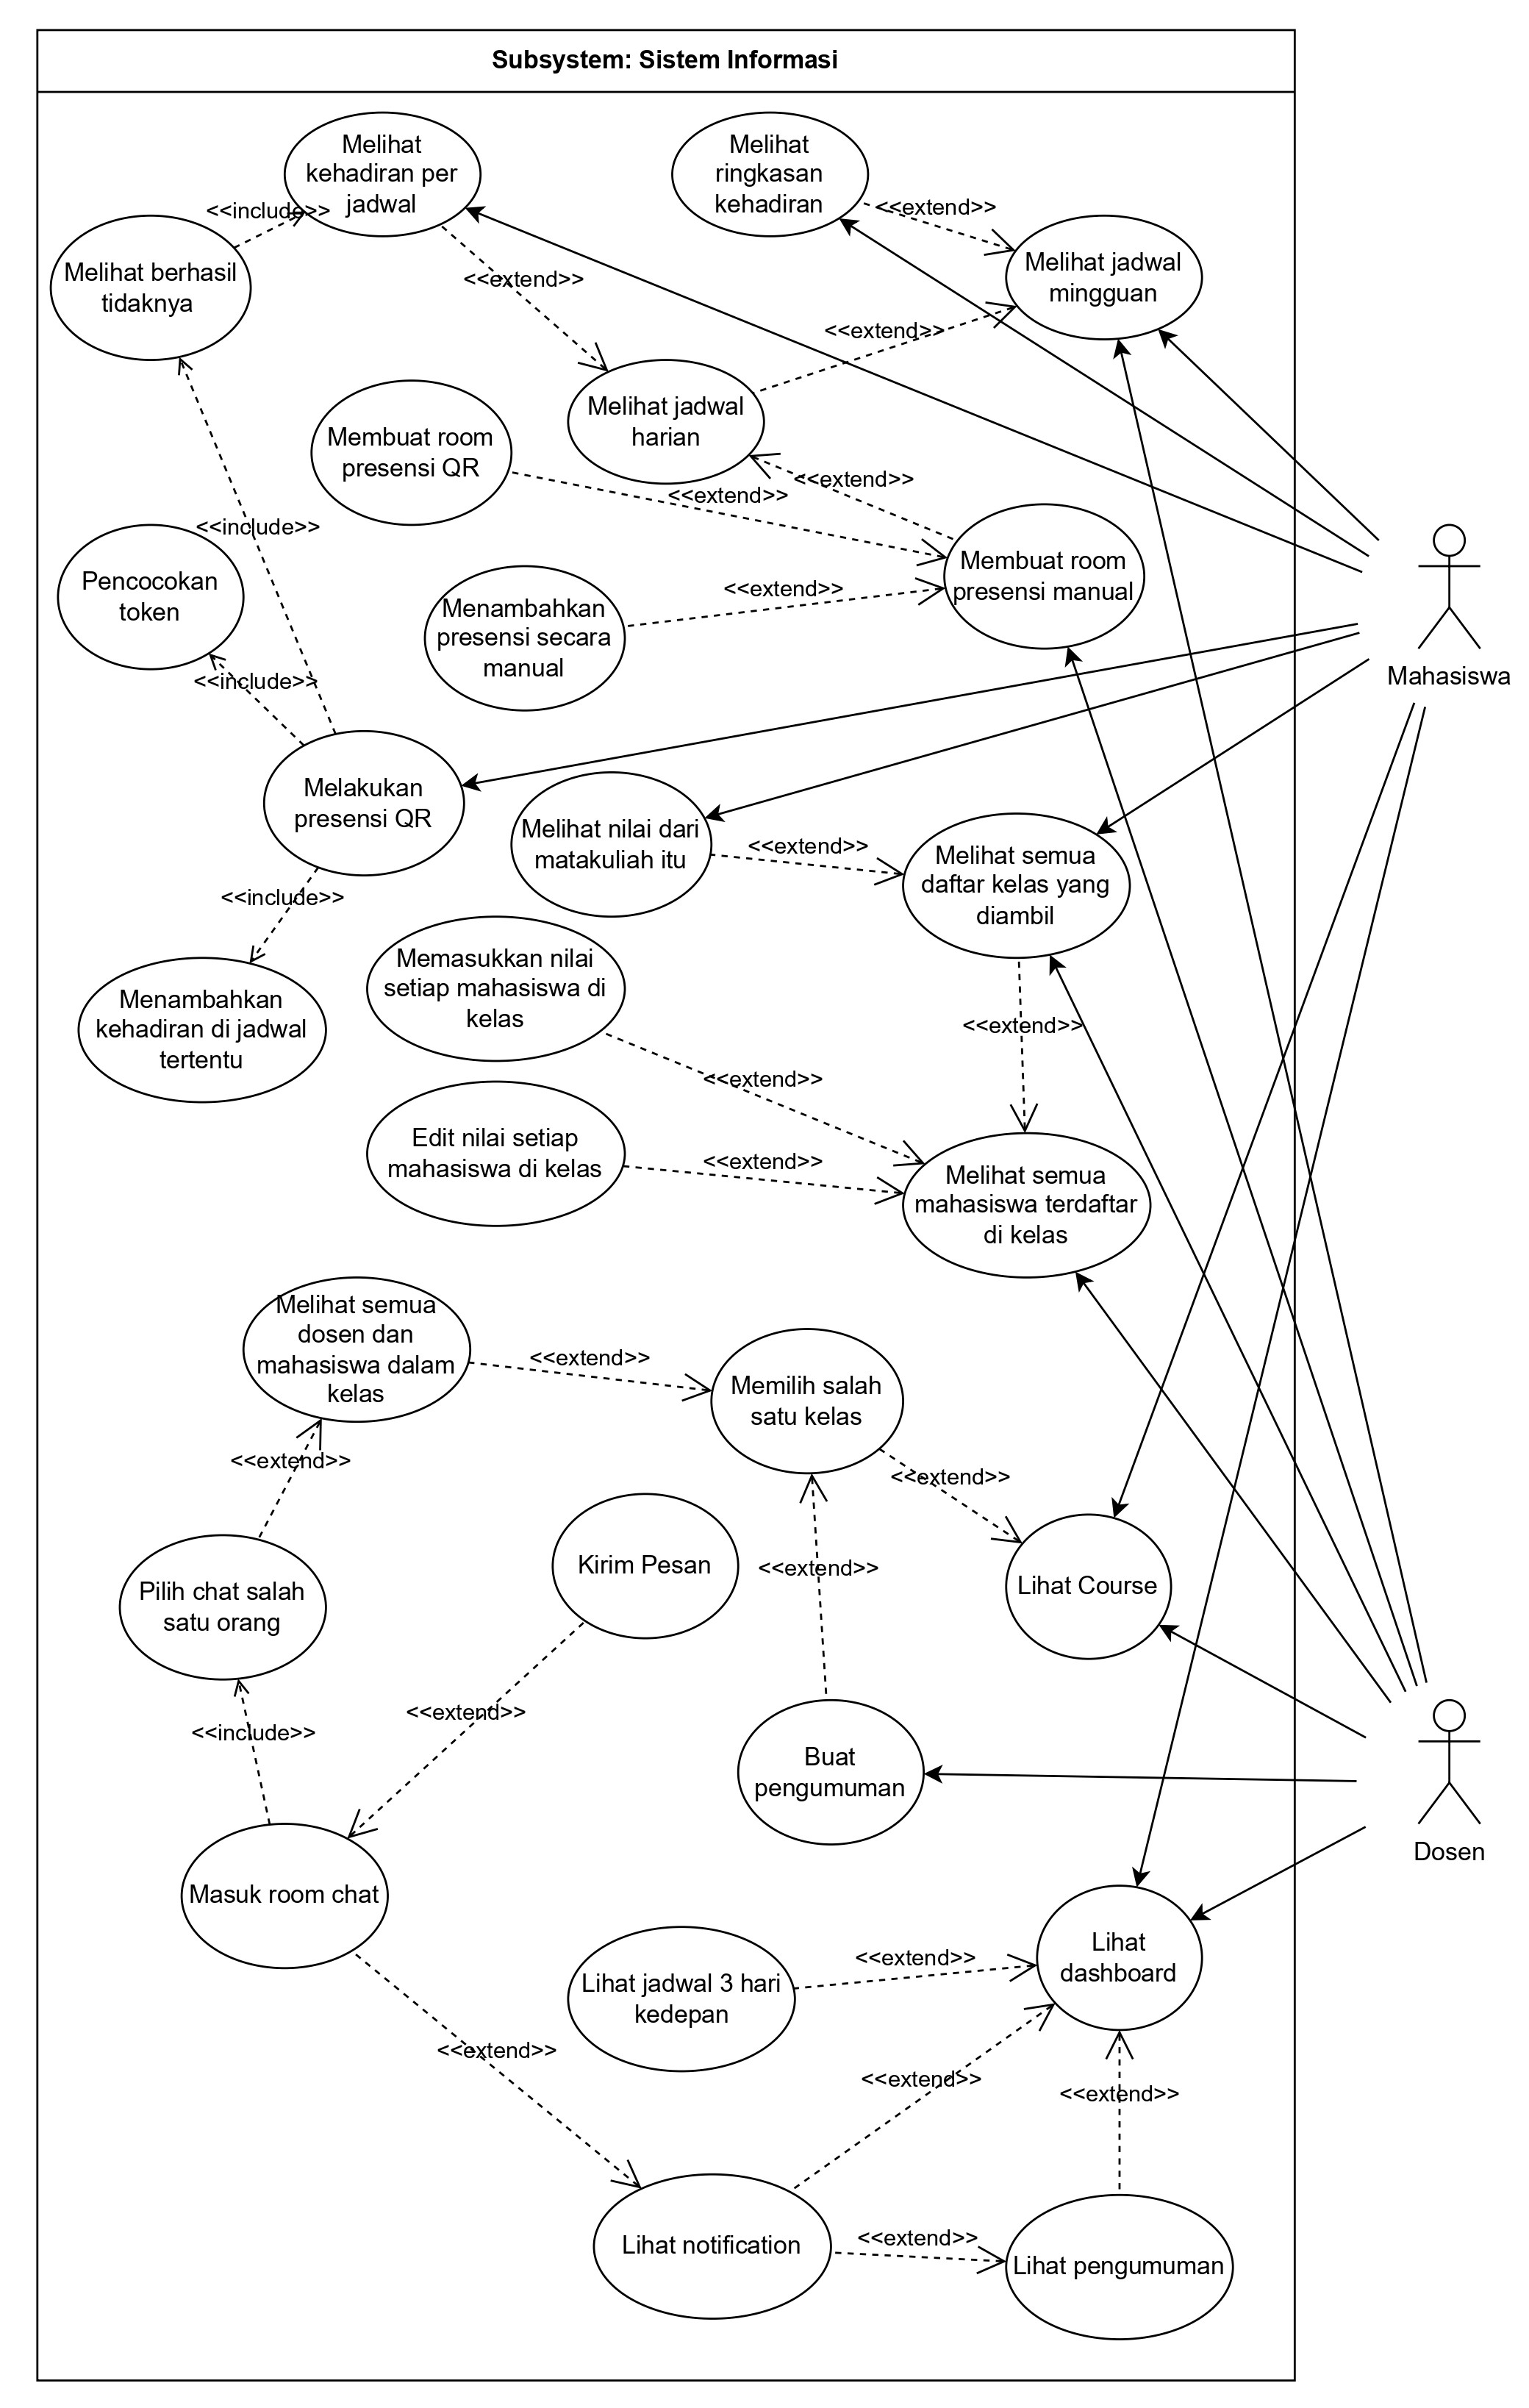
\includegraphics[width=0.8\textwidth]{USECASE/usecaseSistemInformasi.jpg}
  \caption{Use Case Sistem Informasi}
  \label{fig:use_case_sistem_informasi}
\end{figure}

\subsubsection{Penjelasan Use Case Sistem Informasi}

Subsystem Sistem Informasi adalah bagian yang sangat penting dalam sistem akademik modern, karena menyediakan berbagai fitur yang mendukung proses pembelajaran, komunikasi, dan monitoring aktivitas akademik secara digital. Pada diagram use case \ref{fig:use_case_sistem_informasi}, subsystem ini melibatkan dua aktor utama, yaitu Mahasiswa dan Dosen, yang berinteraksi dengan sistem untuk mengakses informasi, melakukan presensi, melihat nilai, berkomunikasi, dan mendapatkan notifikasi terkait aktivitas akademik.

\subsubsection{Aktor dan Peran}

\begin{itemize}
  \item \textbf{Mahasiswa}: Mengakses sistem untuk melihat jadwal, melakukan presensi, melihat nilai, berkomunikasi dengan dosen dan sesama mahasiswa, serta menerima pengumuman dan notifikasi.
  \item \textbf{Dosen}: Mengelola presensi, memasukkan dan mengedit nilai mahasiswa, membuat pengumuman, serta berkomunikasi dengan mahasiswa melalui chat dan notifikasi.
\end{itemize}

\subsubsection{Fitur Utama Subsystem Sistem Informasi}

\begin{enumerate}
  \item \textbf{Presensi QR dan Manual:} Fitur ini memungkinkan mahasiswa untuk melakukan presensi secara digital menggunakan QR code atau secara manual. Dosen dapat membuat room presensi QR atau manual, dan mahasiswa melakukan presensi dengan mencocokkan token atau memasukkan data secara manual. Sistem akan memvalidasi kehadiran dan mencatat status presensi setiap mahasiswa.
  \item \textbf{Monitoring Kehadiran:} Mahasiswa dapat melihat kehadiran per jadwal, ringkasan kehadiran, dan status presensi mingguan maupun harian. Dosen dapat menambahkan kehadiran di jadwal tertentu dan memantau kehadiran mahasiswa secara real-time.
  \item \textbf{Manajemen Nilai:} Dosen dapat memasukkan dan mengedit nilai setiap mahasiswa di kelas. Mahasiswa dapat melihat nilai dari setiap mata kuliah yang diambil. Proses ini terintegrasi dengan daftar kelas dan daftar mahasiswa yang terdaftar di kelas tersebut.
  \item \textbf{Manajemen Kelas dan Course:} Mahasiswa dapat melihat semua daftar kelas yang diambil dan semua mahasiswa yang terdaftar di kelas. Dosen dapat melihat semua dosen dan mahasiswa dalam kelas, serta mengelola course yang diampu.
  \item \textbf{Jadwal dan Dashboard:} Mahasiswa dan dosen dapat melihat jadwal harian, mingguan, dan 3 hari ke depan. Dashboard menyediakan ringkasan aktivitas, jadwal, pengumuman, dan notifikasi yang relevan dengan peran masing-masing aktor.
  \item \textbf{Komunikasi dan Pengumuman:} Fitur chat memungkinkan mahasiswa dan dosen untuk berkomunikasi secara langsung, baik dalam room chat maupun secara personal. Dosen dapat membuat pengumuman yang akan muncul di dashboard dan notifikasi mahasiswa.
  \item \textbf{Notifikasi:} Sistem mengirimkan notifikasi terkait jadwal, pengumuman, dan aktivitas penting lainnya agar mahasiswa dan dosen selalu mendapatkan update terbaru.
\end{enumerate}

\subsubsection{Alur Interaksi Use Case}

Pada diagram use case, terdapat relasi <<include>> dan <<extend>> yang menggambarkan keterkaitan antar fitur. Misalnya, proses melakukan presensi QR selalu melibatkan pencocokan token dan validasi kehadiran. Fitur melihat jadwal harian dan mingguan merupakan perluasan dari fitur monitoring kehadiran. Proses memasukkan dan mengedit nilai mahasiswa di kelas akan terhubung dengan fitur melihat daftar kelas dan mahasiswa yang terdaftar.

Komunikasi antar mahasiswa dan dosen difasilitasi melalui fitur chat, room chat, dan pengumuman. Setiap pengumuman yang dibuat dosen akan muncul di dashboard dan notifikasi mahasiswa, sehingga informasi penting tidak terlewatkan.

\subsubsection{Keamanan dan Efisiensi}

Subsystem ini dirancang untuk memastikan keamanan data akademik, kehadiran, dan nilai mahasiswa. Proses presensi menggunakan QR code dan token untuk mencegah kecurangan. Data nilai dan kehadiran disimpan secara terpusat dan hanya dapat diakses oleh aktor yang berwenang. Notifikasi dan dashboard membantu meningkatkan efisiensi komunikasi dan monitoring aktivitas akademik.

\subsubsection{Contoh Skenario Penggunaan}

\begin{enumerate}
  \item \textbf{Presensi QR Mahasiswa}: Mahasiswa masuk ke room presensi QR, melakukan scan QR code, sistem mencocokkan token dan mencatat kehadiran. Mahasiswa dapat melihat status kehadiran pada jadwal tersebut.
  \item \textbf{Dosen Memasukkan Nilai}: Dosen memilih kelas, memasukkan nilai setiap mahasiswa, dan menyimpan data. Mahasiswa dapat melihat nilai yang telah diinput pada dashboard mereka.
  \item \textbf{Mahasiswa Melihat Jadwal}: Mahasiswa mengakses dashboard untuk melihat jadwal harian, mingguan, dan 3 hari ke depan, serta mendapatkan notifikasi jika ada perubahan jadwal atau pengumuman baru.
  \item \textbf{Chat dan Pengumuman}: Mahasiswa dan dosen masuk ke room chat, memilih salah satu kelas, dan mengirim pesan atau membuat pengumuman yang akan diterima oleh seluruh anggota kelas.
\end{enumerate}

\subsubsection{Kesimpulan}

Subsystem Sistem Informasi merupakan tulang punggung digitalisasi proses akademik di institusi pendidikan. Dengan fitur presensi digital, monitoring kehadiran, manajemen nilai, jadwal, dashboard, komunikasi, dan notifikasi, subsystem ini mendukung kelancaran pembelajaran dan administrasi akademik secara efisien dan aman. Relasi antar fitur dan aktor pada diagram use case memastikan setiap proses berjalan terintegrasi dan sesuai prosedur, sehingga mahasiswa dan dosen dapat fokus pada aktivitas akademik tanpa hambatan teknis. Dengan demikian, subsystem sistem informasi sangat penting untuk mendukung transformasi digital di lingkungan pendidikan modern.


\section{Activity Diagram}
\section{ERD}
\section{Wireframe}

% Progress
\chapter{Progress}
\section{Slicing}
\section{API}
\section{Dokumentasi API}

\end{document}